\section{Experiments}

\begin{figure}
\captionsetup[subfigure]{justification=centering}
  \centering
  \begin{subfigure}{0.24\textwidth}
    \centering
    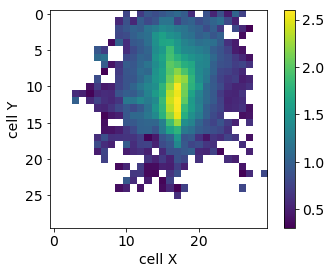
\includegraphics[width=1\textwidth]{figures/1_real.png}
    % \caption{\\$E = 63.7~\text{GeV}$ \\ $\frac{p_x}{p_z}=0.005$ \\ $\frac{p_y}{p_z}=0.154$}\label{fig:real-imgs-1}
  \end{subfigure}
  \begin{subfigure}{0.24\textwidth}
    \centering
    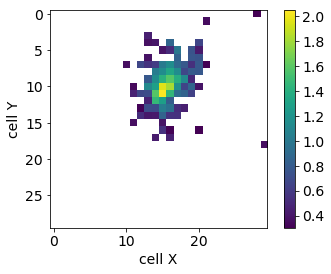
\includegraphics[width=1\textwidth]{figures/2_real.png}
    % \caption{\\$E = 6.5~\text{GeV}$ \\  $\frac{p_x}{p_z}=0.0046$ \\$\frac{p_y}{p_z}=0.108$}\label{fig:real-imgs-2}
  \end{subfigure}
    \begin{subfigure}{0.24\textwidth}
    \centering
    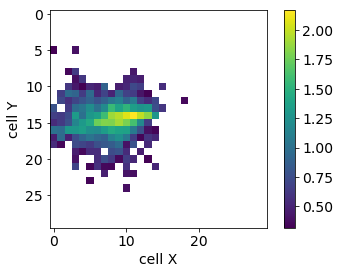
\includegraphics[width=1\textwidth]{figures/3_real.png}
    % \caption{\\$E = 15.6~\text{GeV}$ \\ $\frac{p_x}{p_z}=0.196$ \\ $\frac{p_y}{p_z}=-0.036$}\label{fig:real-imgs-3}
  \end{subfigure}
  \begin{subfigure}{0.24\textwidth}
    \centering
    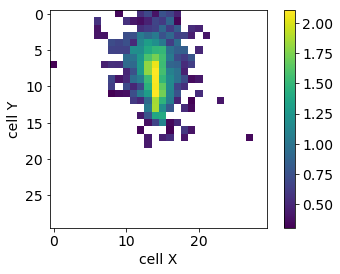
\includegraphics[width=1\textwidth]{figures/4_real.png}
    % \caption{\\$E = 15.6~\text{GeV}$ \\  $\frac{p_x}{p_z}=-0.019$ \\ $\frac{p_y}{p_z}=0.181$}\label{fig:real-imgs-4}
  \end{subfigure}\\
   \begin{subfigure}{0.24\textwidth}
    \centering
    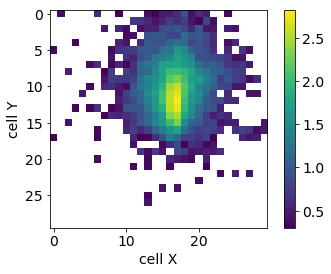
\includegraphics[width=1\textwidth]{figures/1_gen.png}
    \caption{\\$E_0 = 63.7~\text{GeV}$ }%\\ $\frac{p_x}{p_z}=0.005$ ,  $\frac{p_y}{p_z}=0.154$}}%\label{fig:gen-imgs-1}
  \end{subfigure}
  \begin{subfigure}{0.24\textwidth}
    \centering
    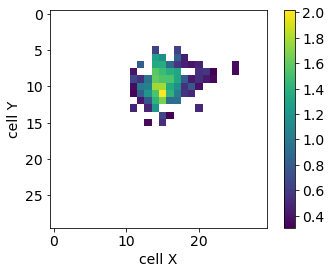
\includegraphics[width=1\textwidth]{figures/2_gen.png}
    \caption{\\$E_0 = 6.5~\text{GeV}$ }% \\  $\frac{p_x}{p_z}=0.046$ , $\frac{p_y}{p_z}=0.108$}}%\label{fig:gen-imgs-2}
  \end{subfigure}
    \begin{subfigure}{0.24\textwidth}
    \centering
    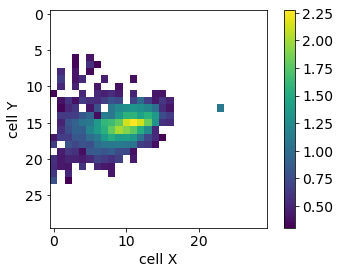
\includegraphics[width=1\textwidth]{figures/3_gen.png}
    \caption{\\$E_0 = 15.6~\text{GeV}$ }% \\ $\frac{p_x}{p_z}=0.196$ ,  $\frac{p_y}{p_z}=-0.036$}}%\label{fig:gen-imgs-3}
  \end{subfigure}
  \begin{subfigure}{0.24\textwidth}
    \centering
    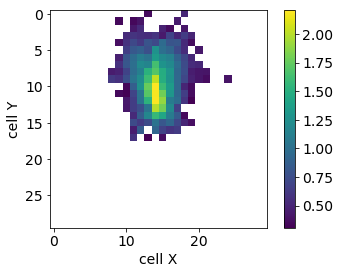
\includegraphics[width=1\textwidth]{figures/4_gen.png}
    \caption{\\$E_0 = 15.9~\text{GeV}$ }% \\  $\frac{p_x}{p_z}=-0.019$ ,  $\frac{p_y}{p_z}=0.181$}}%\label{fig:gen-imgs-4}
  \end{subfigure}
 
  \caption{Showers generated with \geant (first row) and the showers,
    simulated with our model (second row) for three different sets of
    input parameters. Color represents $log_{10}(\frac{E}{MeV})$ for every cell}
  \label{fig:geant_vs_ours}
\end{figure}

We start with comparing original clusters, produced by full \geant
simulation and clusters generated by the trained model for the same
 parameters of the incident particles: the same energy, the same direction,
 and the same position on the calorimeter face. Corresponding images
 for four arbitrary parameter sets are presented
 in~\cref{fig:geant_vs_ours}. These images demonstrate very good
 visual similarity between simulated and generated clusters.


\begin{figure}
  \centering
  \begin{subfigure}[t]{0.3\textwidth}
    \centering
    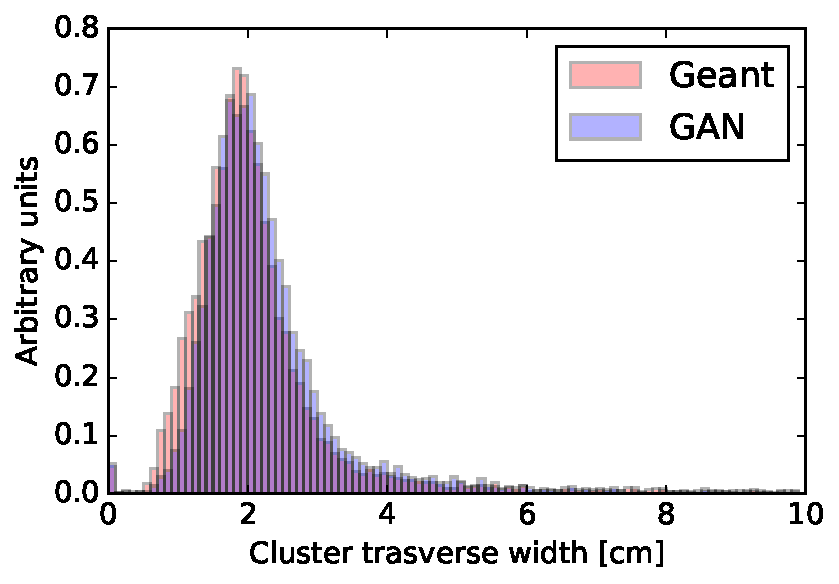
\includegraphics[width=1\textwidth]{figures/width_trans.pdf}
    \caption{The transverse width of real and generated clusters}
  \end{subfigure}\hspace{0.2\textwidth}
 \begin{subfigure}[t]{0.3\textwidth}
    \centering
    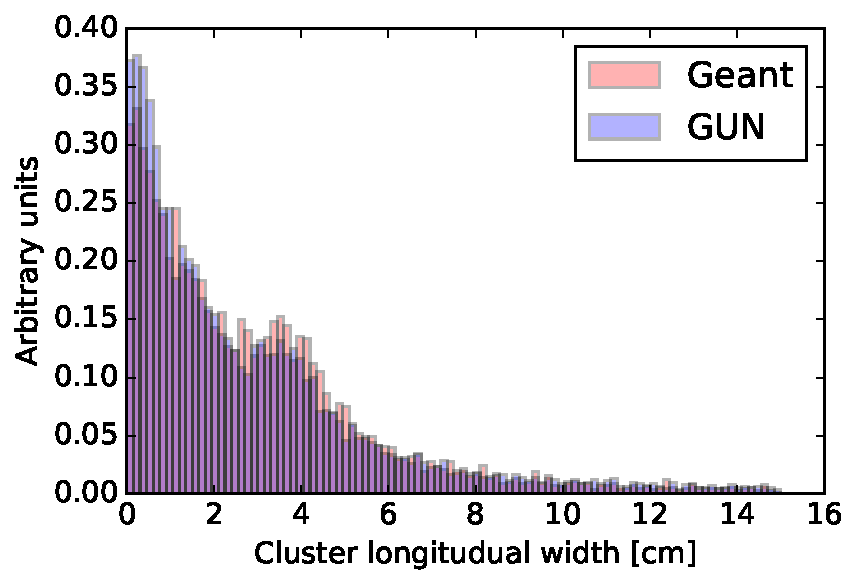
\includegraphics[width=1\textwidth]{figures/width_long.pdf}
    \caption{The longitudinal width of real and generated clusters}
  \end{subfigure}
  \begin{subfigure}[t]{0.3\textwidth}
    \centering
    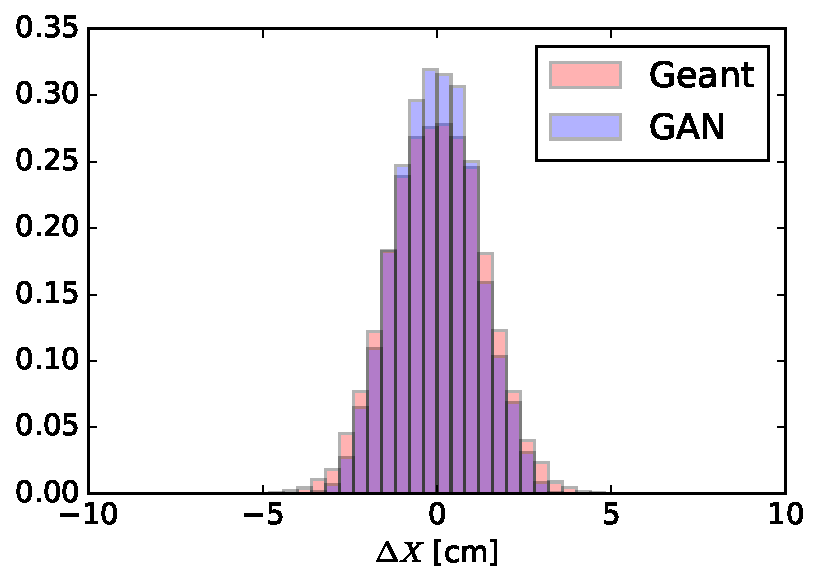
\includegraphics[width=1\textwidth]{figures/deltaX.pdf}
    \caption{$\Delta X$ between cluster center of mass and the true particle coordinate}
  \end{subfigure}\hspace{0.2\textwidth}
  \begin{subfigure}[t]{0.3\textwidth}
    \centering
    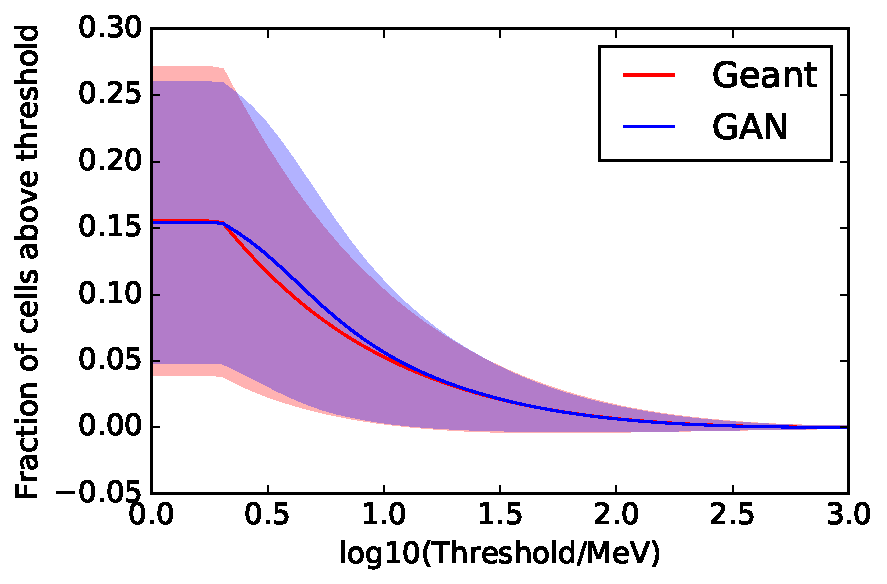
\includegraphics[width=1\textwidth]{figures/sparsity.pdf}
    \caption{The sparsity of real and generated clusters}
  \end{subfigure}
  \begin{subfigure}[t]{0.3\textwidth}
    \centering
    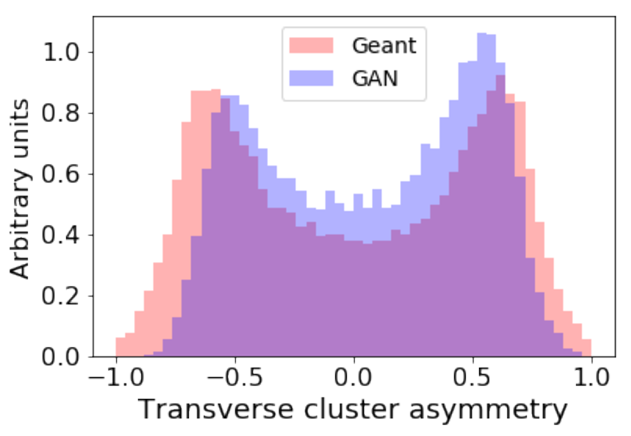
\includegraphics[width=1\textwidth]{figures/transverseAsymmetry.pdf}
    \caption{The transverse asymmetry of real and generated clusters}
  \end{subfigure}\hspace{0.2\textwidth}
  \begin{subfigure}[t]{0.3\textwidth}
    \centering
    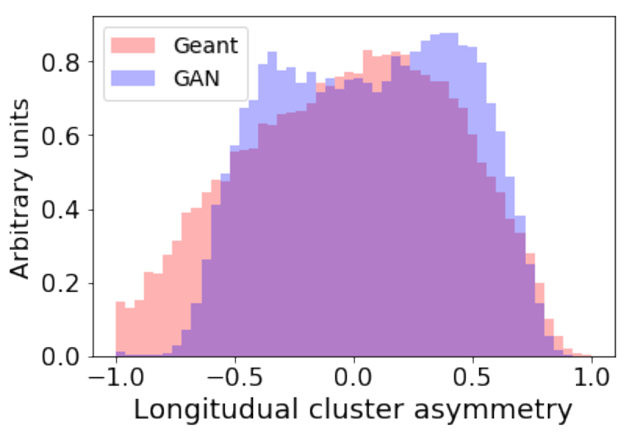
\includegraphics[width=1\textwidth]{figures/longAsymmetry.pdf}
    \caption{The longitudinal asymmetry of real and generated clusters}
  \end{subfigure}
  \caption{Generated images quality evaluation including described physical characteristics.}\label{fig:quality}  
\end{figure}

Then we continue with quantitative evaluation of the proposed simulation
method. While generic evaluation methods for generative models exist,
here we base our evaluation on physics-driven similarity
metrics. These metrics are designed using the domain knowledge and the
recommendations from physicists on the evaluation of simulation
procedures. 
For this presentation we selected few cluster properties which essentially
drive cluster properties used in the reconstruction of calorimeter objects
and following physics analysis. If initial particle direction is not
perpendicular to the calorimeter face, produced cluster is elongated
in that direction. Therefore we consider separately cluster width in
the direction of the initial particle and in the transverse
direction. Spatial resolution, which is the distance between the center
mass of the cluster and the initial track projection to the shower max
depth, is another important characteristics affecting the physics
properties of the cluster. Cluster sparsity, which is the fraction of
cells with energies above some threshold, reflects marginal low
energy properties of the generated clusters. Finally, longitudinal and
transverse asymmetries, which are differences in energies between
forward-backward and left-right sides of the cluster, characterise
coherent energy variations.  
 Comparison of these  characteristics is presented in~\cref{fig:quality}. 

The primary cluster characteristics  demonstrate good agreement with
fully simulated data. However secondary characteristics driven by
long range correlations between different cluster contributions might
be significantly improved.  




As for model performance, we trained our model for 3000 epochs which takes about 70 hours on GPU NVIDIA Tesla K80. The sampling rate is 0.07 ms per sample on GPU, 4.9 ms per sample on CPU.
